\documentclass{article}
\linespread{1.3}
\usepackage[margin=50pt]{geometry}
\usepackage{amsmath, amsthm, amssymb, amsthm, tikz, fancyhdr}
\pagestyle{fancy}
\renewcommand{\headrulewidth}{0pt}
\newcommand{\changefont}{\fontsize{15}{15}\selectfont}

\newcommand{\field}[1]{\mathbb{#1}}
\newcommand{\1}{\mathbf{1}}
\newcommand{\E}{\mathbb{E}} 
\renewcommand{\P}{\mathbb{P}}
\newcommand{\R}{\field{R}} % real domain
% \newcommand{\C}{\field{C}} % complex domain
\newcommand{\F}{\field{F}} % functional domain

\newcommand{\T}{^{\textrm T}} % transpose

\def\diag{\text{diag}}

%% operator in linear algebra, functional analysis
\newcommand{\inner}[2]{#1\cdot #2}
\newcommand{\norm}[1]{\left\|#1\right\|}
\newcommand{\twonorm}[1]{\|#1\|_2^2}
% operator in functios, maps such as M: domain1 --> domain 2
\newcommand{\Map}[1]{\mathcal{#1}}
\renewcommand{\theenumi}{\alph{enumi}} 

\newcommand{\Perp}{\perp \! \! \! \perp}

\newcommand\independent{\protect\mathpalette{\protect\independenT}{\perp}}
\def\independenT#1#2{\mathrel{\rlap{$#1#2$}\mkern2mu{#1#2}}}
\newcommand{\vct}[1]{\boldsymbol{#1}} % vector
\newcommand{\mat}[1]{\boldsymbol{#1}} % matrix
\newcommand{\cst}[1]{\mathsf{#1}} % constant
\newcommand{\ProbOpr}[1]{\mathbb{#1}}
\newcommand{\points}[1]{\small\textcolor{magenta}{\emph{[#1 points]}} \normalsize}
\date{{}}

\fancypagestyle{firstpageheader}
{
  \fancyhead[R]{\changefont Michael Huang \\ CSE 446 \\ Homework 4}
}

\begin{document}

\thispagestyle{firstpageheader}

\section*{A.1}
{\Large 

\subsection*{a.}

True or False: Given a data matrix $X \in \mathbb{R}^{n \times d}$ where $d\ll n$ and $k = \mathrm{rank}(X)$, if we project our data onto a $k$ dimensional subspace using PCA, our projection will have zero reconstruction error (in other words, we find a perfect representation of our data, with no information loss). \\ \\

True? It is possible that if we are given a skinny matrix with $n$ samples $\gg d$ features, we know that the rank $k$ of the matrix can be no larger than its smallest dimension, which in our case will be $d$. This projection of our data using PCA will therefore be pretty useless, since no dimensionality reduction is performed, but it is doable and give us a our original representation of our data sans information loss. 

\subsection*{b.}

True or False: Suppose that a matrix $X\in \mathbb{R}^{n \times n}$ has a singular value decomposition of $USV^{\top}$, where $S$ is a diagonal $n \times n$ matrix. Then, the rows of $V$ are equal to the eigenvectors of $X^{\top}X$. \\ \\

False. The columns of $V$ would be equal to the eigenvectors of $X^T X$, instead.

\subsection*{c.}

True or False: Choosing $k$ to minimize the $k$-means objective (see Equation \eqref{eq:kmeans_obj} below) is a good way to find meaningful clusters. \\ \\

False. We aim to minimize the intra-cluster distance between a given centroid and its clustered points, and for this objective, just choosing a good k isn't necessarily a good  way to minimize this distance overall.


\subsection*{d.}

True or False: The singular value decomposition of a matrix is unique. \\ \\

False. In general, the SVD of a matrix is not unique--if we have repeated singular values, then we can switch around the orders of values in $U$ and $V$.

\subsection*{e.}

True or False: The rank of a square matrix equals the number of its nonzero eigenvalues. \\ \\

False. In general, this is not true. The matrix must be symmetric in order for its rank to equal the number of nonzero eigenvalues.

\subsection*{f.}

True or False: Autoencoders, where the encoder and decoder functions are both neural networks with nonlinear activations, can capture more variance of the data in its encoded representation than PCA using the same number of dimensions. \\ \\

True. PCA uses linear layers in contrast with the non-linear layers of the autoencoder, which are in turn more equipped to capture more features and more variance of the data in its representation.
% False. This is not necessarily the case. For example, with a limited number of dimensions, PCA will still try to seek out variance in its output, while the neural networks might tend to be more overfitted or have less developed layers that could lead to less acclimation to the variance in the data. There are considerations between the linear PCA map and the nonlinear activations with autoencoders as well.

}

\section*{A.2}
{\Large

\subsection*{a.}

\begin{enumerate}
  \item Let $\widehat{w}$ be the solution to the regression problem $\min_{w} \twonorm{Xw - y}$. Let $\widehat{w}_{\rm R}$ be the solution to the ridge regression problem $\min_w \twonorm{X w - y} + \lambda \twonorm{w}$. Let $X = U \Sigma V^\top$ be a singular value decomposition of $X$. Using this decomposition, explain why the solution $\widehat{w}_{\rm R}$ to the ridge regression problem ``shrinks'' as compared to the solution $\widehat{w}$ of the standard regression problem.
  
  The weights in the solution $\widehat{w}_{\rm R}$ to the ridge regression problem ``shrinks'' as compared to the solution $\widehat{w}$ of the standard regression problem since the singular values in the solution to the ridge regression problem are smaller, which are in response to the smaller variance that is achieved. (as is the purpose of using ridge regression over standard regression).
  % small singular values due to lower variance in ridge regression (as is the aim)?
  % I have no clue

  % Yes, using the singular value decomposition of X enables you to prove that the the ridge solution shrinks compared to the standard solution.

  We can use algebra, and express $\widehat{w}$ and $\widehat{w}_{\rm R}$ in terms of the SVD of $X$ and compare their L2-norms: \\ \\
  Standard Regression: \\
  $\min_w \twonorm{X w - y}$ \\
  $= \min_w (Xw - y)^\top(Xw-y)$ \\
  $X\widehat{w} = X (X^\top X)^{-1}X^\top y$ \\
  $= UDV^\top ((UDV^\top)^\top UDV^\top)^{-1}(UDV^\top)^\top y$ \\
  $= UDV^\top (VDU^\top UDV^\top)^{-1}VDU^\top y$ \\
  $= UU^\top y$ \\

  Ridge Regression: \\
  $\min_w \twonorm{X w - y} + \lambda \twonorm{w}$ \\
  $= \min_w (Xw - y)^\top(Xw-y) + \lambda w^\top w$ \\
  $X\widehat{w}_{\rm R} = X(X^\top X + \lambda I)^{-1} X^\top y$ \\
  $= UDV^\top((UDV^\top)^\top UDV^\top + \lambda I)^{-1} (UDV^\top)^\top y$ \\
  $= UDV^\top(VDU^\top UDV^\top + \lambda I)^{-1} VDU^\top y$ \\
  $= UD (D^2 + \lambda I)^{-1} DU^\top y$ \\


  \item Let $U \in \R^{n\times n}$ be a matrix with singular values all equal to one. Show that $UU^\top = U^\top U = I_n$. Further, use this result to show that $U$ preserves Euclidean norms. In other words, $\norm{U x}_2 = \norm{x}_2$ for any $x\in \R^n$. \\
  
  We first use SVD, and show that $UU^\top = I$: \\ 
  $UU^\top = X \Sigma V^\top (X \Sigma V^\top)^\top$ \\
  $= X \Sigma V^\top V \Sigma^\top X^\top$ \\
  $= X \Sigma \Sigma^\top X^\top$ \hfill Orthogonality of $V$, i.e. $V^\top V = I$ \\
  $= X X^\top$ \hfill Singular values in $\Sigma$ all 1, so $\Sigma \Sigma^\top = I I^\top = I$ \\
  $= I$ \hfill Orthogonality of $X$, i.e. $X X^\top = I$ \\ \\
  and that $U^\top U = I$ as well: \\
  $U^\top U = (X \Sigma V^\top)^\top X \Sigma V^\top$ \\
  $= V \Sigma^\top X^\top X \Sigma V^\top$ \\
  $= V \Sigma^\top \Sigma V^\top$ \hfill Orthogonality of $X$, i.e. $X^\top X = I$ \\
  $= V V^\top$ \hfill Singular values in $\Sigma$ all 1, so $\Sigma \Sigma^T = I I^T = I$ \\
  $= I$ \hfill Orthogonality of $V$, i.e. $V V^\top = I$ \\ \\

  We now aim to use this result to show that $U$ preserves Euclidean norms, i.e. $\norm{U x}_2 = \norm{x}_2$ for any $x\in \R^n$: \\
  $\norm{U x}^2_2 = (Ux)^\top Ux$ \hfill By the property that $\norm{x}^2_2 = x^\top x$ \\
  $= x^\top U^\top Ux$ \\
  $= x^\top x$ \hfill Since we showed $U^\top U = I$ \\
  $\norm{U x}^2_2 = \norm{x}^2_2$ \hfill By the aforementioned property \\
  $\norm{U x}_2 = \norm{x}_2$ \hfill Algebra \\


\end{enumerate}

\subsection*{b.}

\begin{enumerate}
  \item 
  We know that $\norm{x}_1 = \sum_{i=1}^{n} |x_i|$, by definition, which we note is both nondifferentiable and convex. Looking at the absolute value terms, we can express each one as $\text{max} \{ g \cdot x_i \}$ where $g \in {-1, 1}$, so we can essentially say that $\norm{x}_1 = \text{max}\{g^\top \cdot x_i\}$. \\ \\
  We can thus find the subgradient set, we first must have $g^\top \cdot x = \norm{x}_1$. Using the absolute value idea as we did previously, we know that for $x_i > 0$, we have $g_i = 1$, while for $x_i < 0$, $g_i = -1$. The only point of interest is at $x_i = 0$, where we can select either $-1$ or $1$ to satisfy the optimization. Our overall set of subgradients can therefore be described as \\
  $\{g \in \norm{g} \leq 1, g^\top \cdot x = \norm{x}_1\}$

  \item $f(x) = \max \left\{f_i(x)\right\}_{i =1}^m$, where $f_i$ are all convex and continuously differentiable functions (i.e., gradients exist everywhere in the domain for $f_i$)
  
  We note that to find the subgradient for the maximum of all the convex and continuously differentiable functions. We can therefore choose some index $i$ such that $f_i(x) = f(x)$, which implies that the subgradient $g \in $ subgradients of $f$. This means that we can simply choose a function within $\left\{f_i(x)\right\}_{i =1}^m$, and then choose any subgradient. 
  % $f(y) \geq f_i(y) \geq f_i(x) + g^\top (y - x) = f(x) + g^\top (y - x)$
  % Convex hull thing 

\end{enumerate}

\subsection*{c.}

In this subproblem, you will need to use the result of part b above. Consider the function $f(x) = \max_{i = 1, 2, \dots, n} |x_i - (1 + \eta/i)|$ for some constant $\eta$. Let $v$ be any subgradient of $f$ at any point in its domain. What is the best upper bound you can prove on $\norm{v}_{\infty}$? \\

$f(x) = \max_{i = 1, 2, \dots, n} |x_i - (1 + \eta/i)|$
% Apply this elementwise

}

\section*{A.3}
{\Large 

\subsection*{a.}

$\lambda_1 = 5.116787728342086$ \\
$\lambda_2 = 3.741328478864837$ \\
$\lambda_{10} = 1.2427293764173342$ \\
$\lambda_{30} = 0.364255720278894$ \\
$\lambda_{50} = 0.16970842700672767$ \\
$\sum_{i=1}^d{\lambda_i} = 52.72503549512691$

\subsection*{b.}

% Any example $x \in \mathbb{R}^d$ (including those from either the training or test set) can be approximated using just $\mu$ and the first $k$ eigenvalue, eigenvector pairs, for any $k = 1, 2, \ldots, d$. For any $k$, provide a formula for computing this approximation. \\

In terms of the first $k$ eigenvectors $V_k$, we can use what we have been doing so far, and adjusting for the mean value: \\
$V_k^\top V_k (x - \mu) + \mu$
% not sure if this perfectly captures 

\subsection*{c.}

\begin{figure}[h]
  \centering
  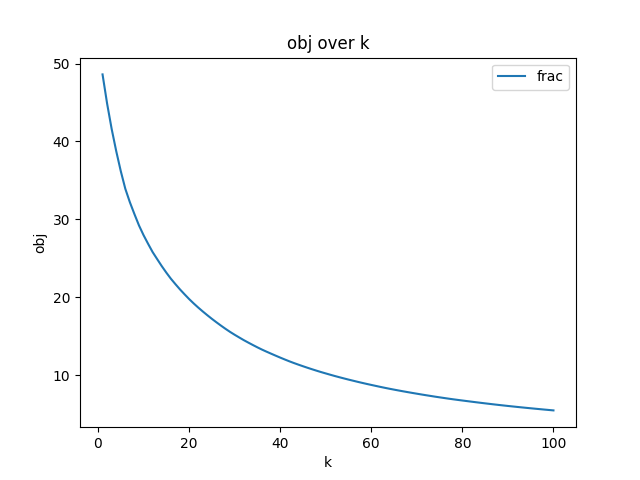
\includegraphics[width=130mm]{../hw4-code/results/a3_cobj.png}
\end{figure}

\begin{figure}[h]
  \centering
  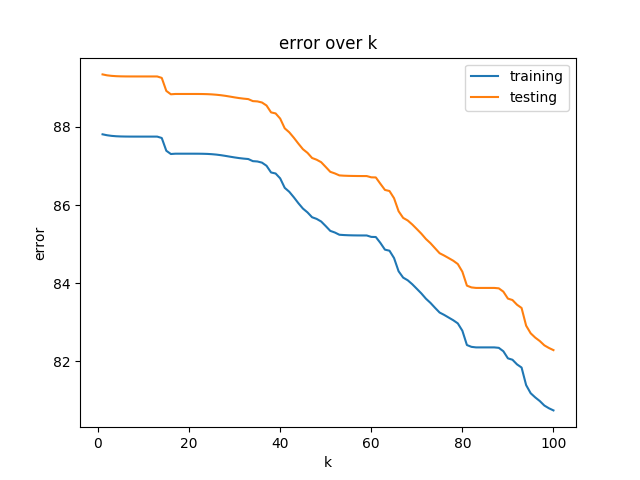
\includegraphics[width=130mm]{../hw4-code/results/a3_cerr.png}
\end{figure}

\newpage

\subsection*{d.}

% Now let us get a sense of what the top PCA directions are capturing. Display the first $10$ eigenvectors as images, and provide a brief interpretation of what you think they capture.

\begin{figure}[!hb]
  \centering
  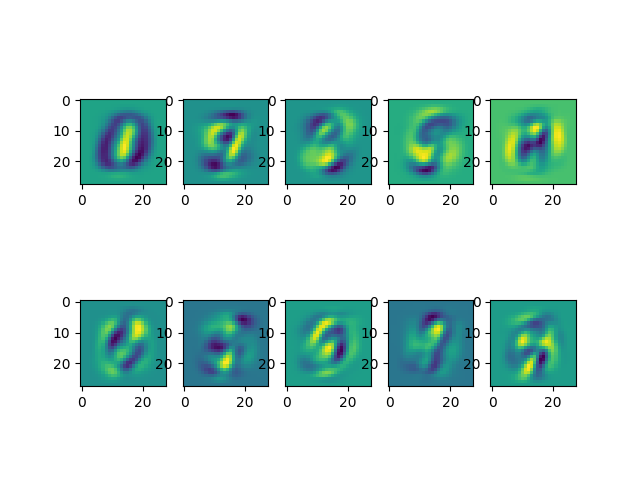
\includegraphics[width=130mm]{../hw4-code/results/a3_d.png}
\end{figure}

The first 10 eigenvectors are essentially trying to capture the most core visual elements of a number, or the most distinguishing features that a person can generally use to pick out and easily categorize any given digit. Each component essentially captures the most variation in the data, which provides the most information for reconstructing the image.

\subsection*{e.}

% Finally, visualize a set of reconstructed digits from the training set for different values of $k$. In particular provide the reconstructions for digits $2, 6, 7$ with values $k = 5, 15, 40, 100$ (just choose an image from each digit arbitrarily). Show the original image side-by-side with its reconstruction. Provide a brief interpretation, in terms of your perceptions of the quality of these reconstructions and the dimensionality you used.

\begin{figure}[!hb]
  \centering
  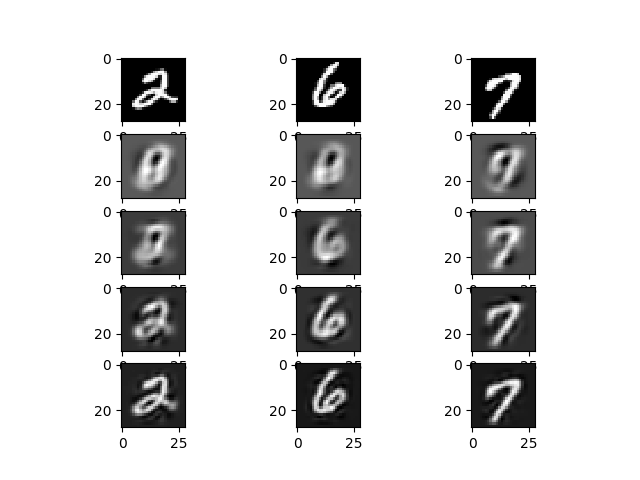
\includegraphics[width=130mm]{../hw4-code/results/a3_e.png}
\end{figure}

With more of the top eigenvectors, the image interpretation of each digit becomes much clearer. The digit becomes clearer with greater dimensionality, with the top 40 eigenvectors being good enough to tell each digit for sure, and just the first 15 eigenvectors being good enough to interpret for 6 and 7, and guessable for 2.

}

\section*{}
{\Large 

\newpage

\begin{verbatim}
# pca.py
# Applicable helpers for HW4 A3

import pandas as pd
import matplotlib.pyplot as plt
import numpy as np

import constants as c
import helpers as h

from mnist import MNIST
from scipy import linalg

def part_a(X, mu=None):
  n, d = X.shape

  if mu is None:
    mu = np.mean(X, axis=0)

  diff = X - mu
  sigma = np.matmul(diff.T, diff) / n

  lamb, v = np.linalg.eig(sigma)
  lamb = lamb.real
  v = v.real

  return lamb, v

def part_c(X_train, X_test):
  train_mse_data = []
  test_mse_data = []
  frac_data = []
  
  e_train, v_train = part_a(X_train)

  for i in range(c.k):
    recon_train = (v_train[:, :i+1]).dot(v_train[:, :i+1].T)
    recon_test = recon_train.dot(X_test.T).T
    recon_train = recon_train.dot(X_train.T).T

    mse_train = np.sum(np.square(recon_train - X_train)) / X_train.shape[0]
    mse_test = np.sum(np.square(recon_test - X_test)) / X_test.shape[0]
    
    train_mse_data.append(mse_train)
    test_mse_data.append(mse_test)

    frac = 1 - (np.sum(e_train[:i+1]) - np.sum(e_train))

    frac_data.append(frac)

  return train_mse_data, test_mse_data, frac_data

def part_d(v_list):
  fig, axes = plt.subplots(2, 5)

  axes_list = []
  for i, item in enumerate(axes):
    axes_list += list(item)

  for i, ax in enumerate(axes_list):
    img = v_list[:,i].reshape((28, 28))
    ax.imshow(img, cmap='gray')

  fig.savefig(c.results_path + "a3_d")

def part_e(X_train, v_list):
  # for 2, 6, 7
  idx_set = [5, 13, 15]
  k_set = [5, 15, 40, 100]
  final_set = [X_train[idx_set[i], :] for i, _ in enumerate(idx_set)]

  for k in k_set:
    for idx in idx_set:
      image = (v_list[:, :k]).dot(v_list[:, :k].T)
      image = image.dot(X_train.T).T
      final_set.append(image[idx])

  fig, axes = plt.subplots(5, len(idx_set))

  for i, ax in enumerate(axes.ravel()):
    ax.imshow(final_set[i].reshape((28, 28)), cmap='gray')

  fig.savefig(c.results_path + "a3_e")

def main():
  output = open(c.results_path + "a3.txt", "w")

  X_train, X_test = h.load_mnist()

  e_list, v_list = part_a(X_train)
  output.write(str([e_list[0], e_list[1], e_list[9],
                   e_list[29], e_list[49]]) + "\n")
  output.write(str(sum(e_list)) + "\n")

  train_mse_data, test_mse_data, frac_data = part_c(
      X_train, X_test)
  h.plot_multiple("error over k", "a3_cerr", "k", "error", 
                  [train_mse_data, test_mse_data], c.tt_list)
  h.plot_multiple("obj over k", "a3_cobj", "k", "obj", 
                  [frac_data], ["frac"])

  part_d(v_list) 

  part_e(X_train, v_list)

  output.close()


if __name__ == "__main__":
  main()

\end{verbatim}

\begin{verbatim}
# helpers.py
# Applicable helpers for HW3

import pandas as pd
import matplotlib.pyplot as plt
import numpy as np

import constants as c

from mnist import MNIST
from scipy import linalg

"""
Helper function for loading in MNIST data set
"""

def load_mnist():
  # load data
  mndata = MNIST(c.data_path)

  X_train, labels_train = map(np.array, mndata.load_training())
  X_test, labels_test = map(np.array, mndata.load_testing())
  X_train = X_train/255.0
  X_test = X_test/255.0

  return X_train, X_test

"""
Helper function for plotting multiple functions
"""
def plot_multiple(plt_title, img_title, x_label, y_label, data_list, legend_list):
  
  assert (len(data_list) > 0)

  iterations = list(range(1, len(data_list[0]) + 1))

  for data in data_list:
    plt.plot(iterations, data)

  plt.title(plt_title)
  plt.xlabel(x_label)
  plt.ylabel(y_label)
  plt.legend(legend_list)

  plt.savefig(c.results_path + img_title + c.png_exten)
  plt.close()

\end{verbatim}

\begin{verbatim}
# constants.py
# Applicable constants for HW4

import numpy as np
import os

home_dir_path = os.path.dirname(os.path.dirname(os.path.abspath(__file__)))

data_path = home_dir_path + '/data/'
results_path = home_dir_path + '/results/'

png_exten = '.png'

d = 784
k = 100

tt_list = ["training", "testing"]
\end{verbatim}

\newpage

}

\section*{A.4}
{\Large 

In this exercise, we will train two simple autoencoders to perform
dimensionality reduction on MNIST. As discussed in lecture, autoencoders are a
long-studied neural network architecture comprised of an encoder component to
summarize the latent features of input data, and a decoder component to try and
reconstruct the original data from the latent features. \\ \\

We recommend using \texttt{nn.Linear} for your linear layers. You will not need to initialize the weights yourself; the default He/Kaiming uniform initialization in PyTorch will be sufficient. \emph{Hint: we also recommend using the \text{\texttt{nn.Sequential}} module to organize your
network class and simplify the process of writing the forward pass.} \\ \\

Use \texttt{optim.Adam} for this question. Experiment with different learning rates. Use mean
squared error (\texttt{nn.MSELoss()} or \texttt{F.mse\_loss()}) for the loss function and ReLU for the non-linearity in b.

\subsection*{a.}

Use a network with a single linear layer. Let $W_{\rm e} \in \mathbb{R}^{h \times d}$ and
    $W_{\rm d} \in \mathbb{R}^{d\times h}$. Given some $x \in \mathbb{R}^d$,
    the forward pass is formulated as
    \[
      \mathcal{F}_{1}(x) = W_{\rm d} W_{\rm e} x\ .
    \]
    Run experiments for $h \in \{ 32, 64, 128 \}$. For each of the different $h$ values, report your final error and visualize a set of $10$ reconstructed digits, side-by-side with the original image. \emph{Note:} We omit the bias term in the formulation for notational convenience since \texttt{nn.Linear} learns bias parameters alongside weight parameters by default.

\subsection*{b.}

Use a single-layer network with non-linearity. Let $W_{\rm e} \in \mathbb{R}^{h \times d}$, $W_{\rm d} \in \mathbb{R}^{d\times h}$, and activation $\sigma\colon \mathbb{R} \to \mathbb{R}$. Given some $x \in \mathbb{R}^d$, the forward pass is formulated as 
    \[
      \mathcal{F}_{2}(x) = \sigma\left(W_{\rm d} \sigma\left(W_{\rm e} x\right)\right)\ .
    \]
    Report the same findings as asked for in part a (for $h \in \{ 32, 64, 128 \}$.

\subsection*{c.}

Now, evaluate $\mathcal{F}_1(x)$ and $\mathcal{F}_2(x)$ (use $h = 128$     here) on the test set. Provide the test reconstruction errors in a table.

\subsection*{d.}

In a few sentences, compare the quality of the reconstructions from these two autoencoders compare with those of PCA from last assignment. You may want to re-run your code for PCA using the different $h$ values as the number of top-$k$ eigenvalues.

}

\section*{A.5}
{\Large 

Given a dataset $x_1, \dots, x_n \in \R^{d}$ and an integer $1 \leq k \leq n$, recall the following $k$-means objective function
\begin{align}
    \min_{\pi_1, \ldots, \pi_k} \sum_{i=1}^{k} \sum_{j \in \pi_i} \norm{ x_j - \mu_{i} }^2_2 \ , \quad \mu_i = \frac{1}{|\pi_i|} \sum_{j \in \pi_i} x_j \ . \label{eq:kmeans_obj}
\end{align}
Above, $\{\pi_i\}_{i=1}^{k}$ is a partition of $\{1, 2, \ldots, n\}$. The objective \eqref{eq:kmeans_obj} is NP-hard\footnote{To be more precise, it is both NP-hard in $d$ when $k=2$ and $k$ when $d=2$. See the references on the Wikipedia page for $k$-means for more details.} to find a global minimizer of. Nevertheless Lloyd's algorithm, the commonly-used heuristic which we discussed in lecture, typically works well in practice.

\subsection*{a.}

Implement Lloyd's algorithm for solving the $k$-means objective \eqref{eq:kmeans_obj}. Do not use any off-the-shelf implementations, such as those found in \texttt{scikit-learn}. Include your code in your submission.

\subsection*{b.}

Run the algorithm on the \emph{training} dataset of MNIST with $k=10$, plotting the objective function \eqref{eq:kmeans_obj} as a function of the iteration number. Visualize (and include in your report) the cluster centers as a $28\times 28$ image.

\subsection*{c.}

For $k=\{2, 4, 8, 16, 32, 64\}$ run the algorithm on the \emph{training} dataset to obtain centers $\{\mu_{i}\}_{i=1}^k$. If $\left\{\left(x_i,y_i\right)\right\}_{i=1}^n$ and $\left\{\left(x_i',y_i'\right)\right\}_{i=1}^m$ denote the training and test sets, respectively, plot the training error $\frac{1}{n} \sum_{i=1}^n \min_{j=1,\dots,k} \twonorm{ \mu_j - x_i }$ and test error $\frac{1}{m} \sum_{i=1}^m \min_{j=1,\dots,k} \twonorm{ \mu_j - x_i' }$ as a function of $k$ on the same plot.

}

\section*{A.6}
{\Large 

In this question, you will explore how to apply machine learning theory and techniques to real-world problems. Each of the following statements details a setting, a dataset and a specific result we hope to achieve. Your job is to briefly (4-7 sentences) describe how you, if tasked with each of the below, would handle this scenario with the tools we’ve learned in this class. \\ \\
Your response should include any pre-processing steps you would take (i.e., data processing / acquisition), the specific machine learning pipeline you would use (i.e., algorithms and techniques learned in this class), and how your setup acknowledges the constraints and achieves the desired result. You should also aim to leverage some of the theory we have covered in this class. Some things to consider may be: the nature of the data (i.e., How hard is it to learn? Do we need more data? Are the data sources good?), the effectiveness of the pipeline (i.e., How strong is the model when properly trained and tuned?), and the time needed to effectively perform the pipeline. \\ \\
Because of the open-ended nature of the question, any thoroughly written responses will receive full credit.

\subsection*{a.}

Small scale image classification \\ \\
\begin{itemize}
    \item Setting: You are tasked by a research institute to create an algorithm that learns the factors that contribute most to acquiring a specific disease.
    \item Dataset: A rich dataset of personal demographic information, location information, risk factors, and whether a person has the disease or not.
    \item Result: The company wants a system that when someone enters their information can determine how susceptible they are to this disease. The pipeline should take limited amount of personal data from a new user and infer more detailed metrics about the person.
\end{itemize}



\subsection*{b.}

Social Media App Facial Recognition Technology \\ \\
\begin{itemize}
    \item Setting: You are tasked with developing a machine learning pipeline that can quickly map someone’s face for the application of filters (i.e., Snapchat, Instagram).
    \item Dataset: A set of face images compiled from the company’s employees and their families.
    \item  Result: The company wants an algorithm that can quickly identify the key features of a person’s face to apply a filter. (Do not worry about describing the actual filter application!).
\end{itemize}



\subsection*{c.}

Malware Detection \\ \\
\begin{itemize}
    \item Setting: You are tasked by a major tech company to create a service that ingests malware metadata and provides accurate assessments as to whether a new file is malicious or not.
    \item Dataset: A set of malware file metadata from users worldwide describing all attributes of offending files including its contents, publisher, and attributes of the resultant activity.
    \item Result: The company wants an accurate, scalable solution to detect whether incoming files are malicious for users across the globe.
\end{itemize}



}

\end{document}